\section{Танилцуулга}
Миний дадлагын хугацаанд ажилсан систем нь хиймэл оюун ухаан, машин сургалтын технологийг ашиглан бүх төрлийн шошгыг хэрэглэгчийн оруулсан мэдээллийг ашиглан үүсгэдэг систем юм. Ингэснээр дизайнер хүмүүсийн ажлыг хөнгөвчилж байгаа билээ. Энэхүү систем нь recommendation model ашиглан ямар төрлийн хүмүүст зориулснаар нь ялгаж өөр төрлийн хэв маягийн өнгө, зураг, дизайн сонгодог ба тэрхүү сонгодогсон матералуудыг LAYOUTGAN++ гэх model ашиглан layout-г нь тохируулж эцсийн бүтээгдэхүүнийг үүсгэдэг.
\section{Use-case диаграм}
\begin{figure}[h]
	\centering
	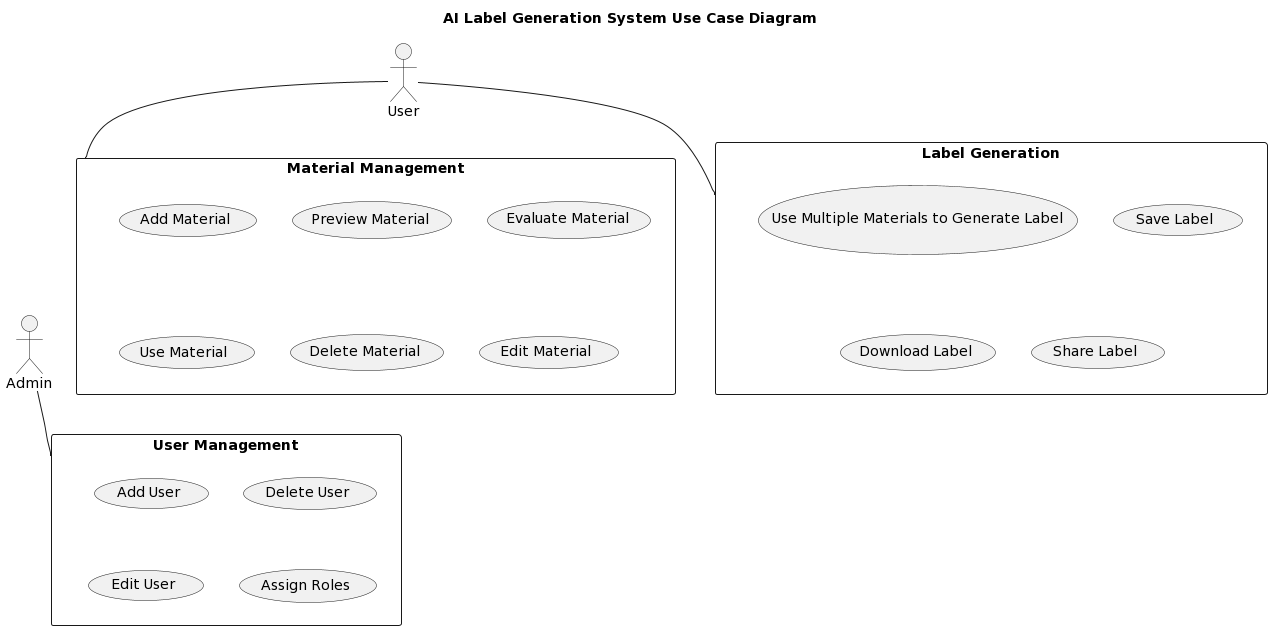
\includegraphics[scale=0.4]{src/pictures/usecase.png}
	\caption{Use-case диаграм}
\end{figure}
\section{Функционал шаардлагууд}
\begin{itemize}
	\item \textbf{Хэрэглэгчийн бүртгэл}: Вэбсайт нь хэрэглэгчдэд цахим шуудангийн хаягаа ашиглан бүртгүүлэх, бүртгэл үүсгэх боломжийг олгох ёстой.

	\item \textbf{Хэрэглэгчийн нэвтрэлт}: Бүртгэгдсэн хэрэглэгчид бүртгүүлсэн цахим шуудан болон нууц үгээ ашиглан бүртгэлдээ нэвтрэх боломжтой байх ёстой.

	\item \textbf{Хэрэглэгчийн хяналтын самбар}: Нэвтэрсэний дараа хэрэглэгч өөрийн профайлыг удирдах, шошго үүсгэх функцэд хандах боломжтой хяналтын самбартай байх ёстой.

	\item \textbf{Зураг байршуулах}: Хэрэглэгчид шошго үүсгэхийг хүссэн зургаа байршуулах боломжтой байх ёстой (adobe illustrator file ашиглах ёстой).

	\item \textbf{Машин сургалтын model ашиглах endpoint}: Вэбсайт нь байршуулсан зураг дээр үндэслэн шошго үүсгэх боломжтой endpoint-уудтай байх ёстой.

	\item \textbf{Шошго үүсгэх}: Зургийг байршуулсны дараа вэбсайт нь машин сургалтын model ашиглан шошго үүсгэх ёстой.

	\item \textbf{Шошгоны дэлгэц}: Вэбсайт нь үүсгэсэн шошгыг хэрэглэгчдэд харуулах ёстой.

	\item \textbf{Шошго татаж авах}: Хэрэглэгчид үүсгэсэн шошгыг тохирох форматаар татаж авах боломжтой байх ёстой (AI эсвэл PNG).

	\item \textbf{Хэрэглэгчийн санал хүсэлт}: Хэрэглэгчид үүсгэсэн шошгоны нарийвчлалын талаар санал хүсэлт өгөх боломжтой байх ёстой.
\end{itemize}
\section{Функционал бус шаардлагууд}
\begin{itemize}
	\item \textbf{Хурд}: Шошго үүсгэх үйл явц нь хамгийн бага хоцрогдолтой, хурдан бөгөөд үр дүнтэй байх ёстой.

	\item \textbf{Аюулгүй байдал}: Хэрэглэгчийн мэдээлэл, үүнд байршуулсан зураг, хамгаалагдсан байх ёстой.

	\item \textbf{Өргөтгөх чадвар (Scalibility)}: Вэбсайт нь хурд алдагдуулахгүйгээр олон тооны хэрэглэгчдэд үйлчлэх чадвартай байх ёстой.

	\item \textbf{Ашиглах боломж}: Вэбсайт нь хэрэглэгчдэд ээлтэй интерфэйстэй, ойлгомжтой зааварчилгаа, хялбар навигацтай байх ёстой.

	\item \textbf{Найдвартай байдал}: Шошго үүсгэхэд ашигладаг машин сургалтын model нь үнэн зөв, найдвартай үр дүнг өгөх ёстой.

	\item \textbf{Хүртээмжтэй байдал}: Вэбсайт нь өөр өөр хөтөч (Chrome, Firefox, Safari гэх мэт) болон төхөөрөмжүүдтэй (ширээний компьютер, гар утас, таблет) нийцтэй байх ёстой.

	\item \textbf{Maintainibility}: Вэбсайт болон түүний үндсэн код нь засвар үйлчилгээ хийх, шинэчлэхэд хялбар байх ёстой.

	\item \textbf{Дагаж мөрдөх}: Вэбсайт нь өгөгдөл хамгаалах хууль, дүрэм журамд нийцсэн байх ёстой.
\end{itemize}

\section{ER диаграм}
\begin{figure}[h!]
	\centering
	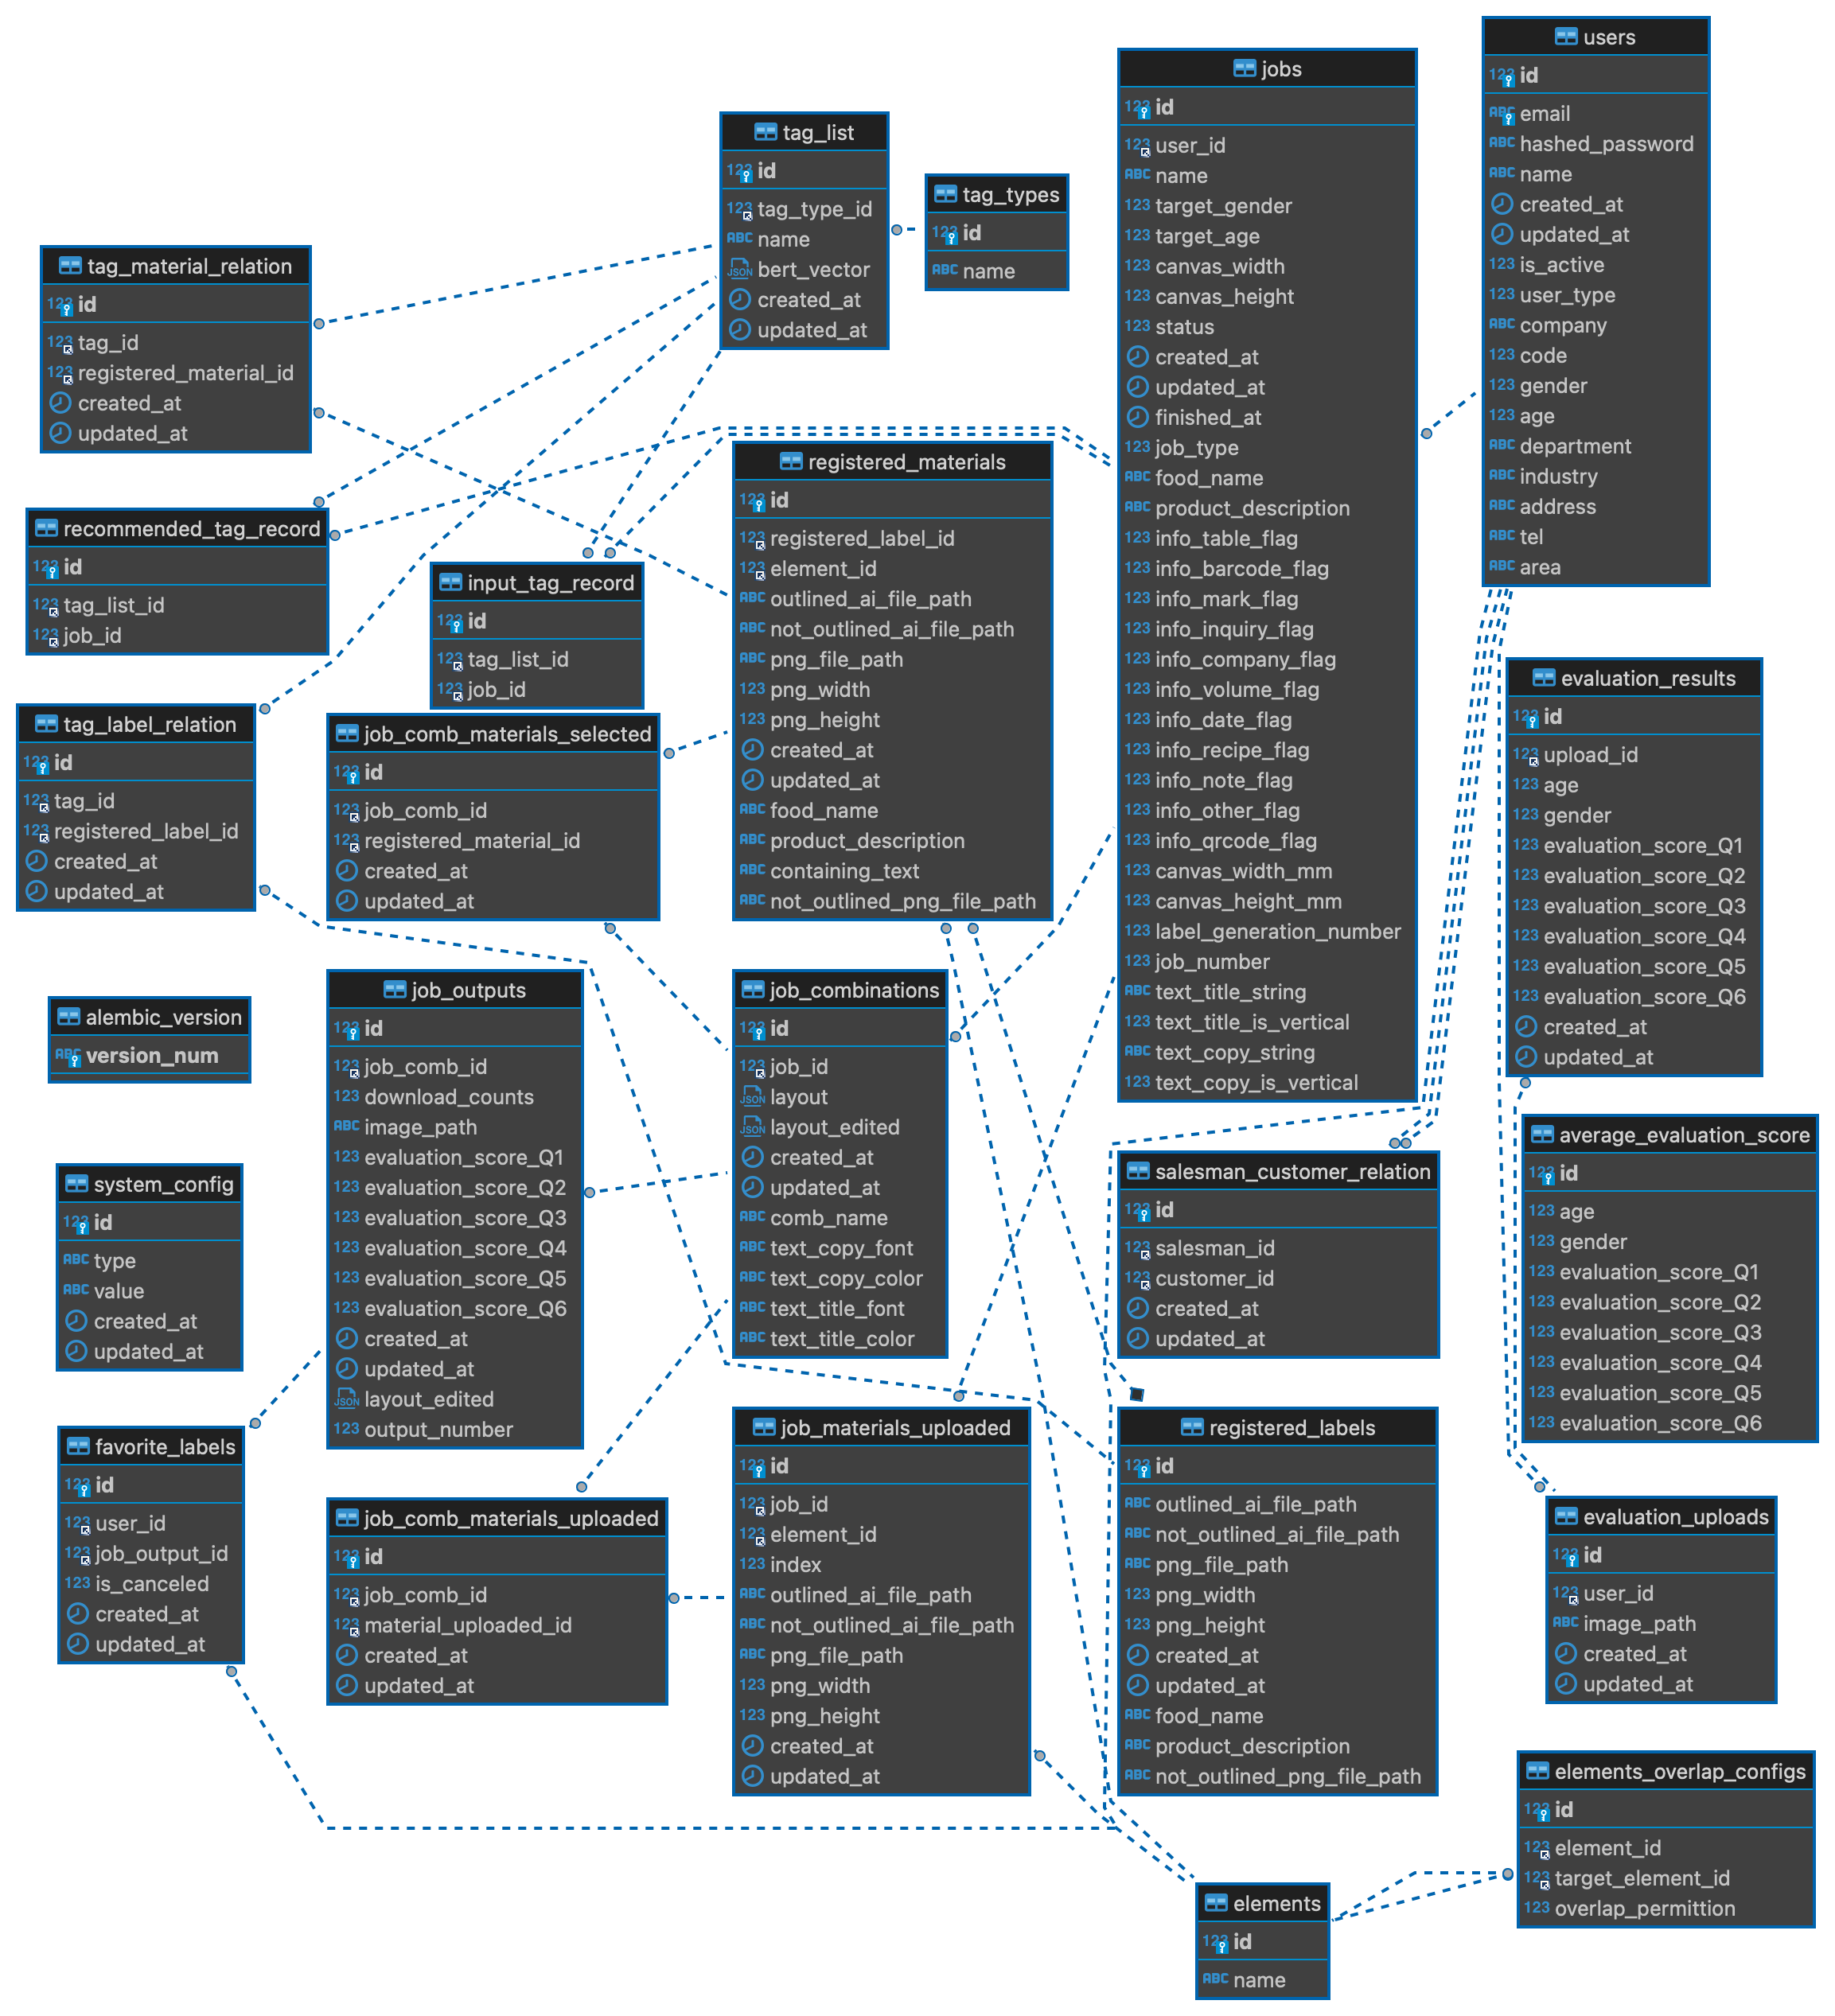
\includegraphics[scale=0.2]{src/pictures/erd.png}
	\caption{Entity relation диаграм}
\end{figure}
\section{Sequence диаграм}

\begin{figure}[h!]
	\centering
	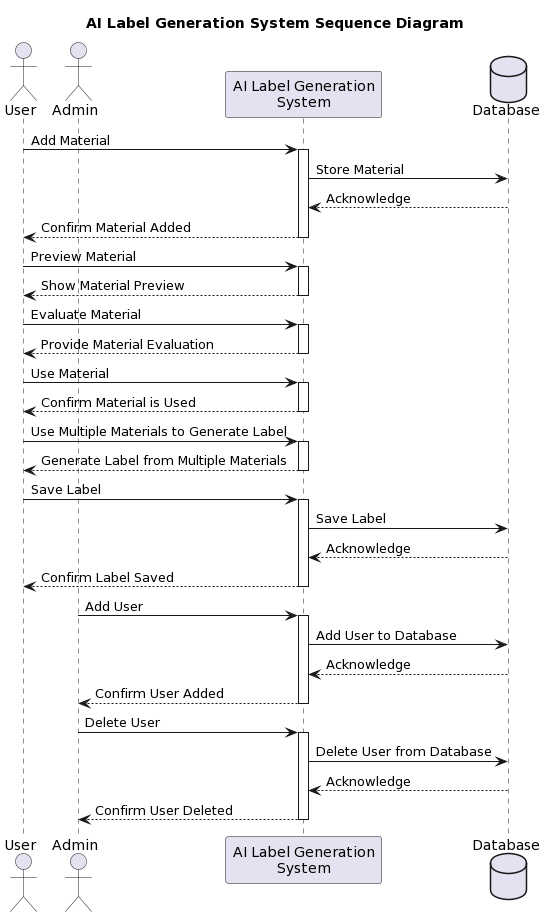
\includegraphics[scale=0.6]{src/pictures/sequence_diagram.png}
	\caption{Sequence диаграм}
\end{figure}